\documentclass[sigconf, 7pt]{acmart}

\usepackage{graphicx}
\usepackage{stfloats}

\settopmatter{printacmref=false} % Removes citation information below abstract
\renewcommand\footnotetextcopyrightpermission[1]{} % removes footnote with conference information in first column
\pagestyle{plain} % removes running headers

\title{\textbf{Exploring the Optimization of the Non-Quadratic Sphere}}
\author{Ravinder Rai}
\date{\today}


\begin{document} 



\begin{abstract}
Using the Matlab function fminunc, we explore the problem of finding the minimum value of a specific variant of the sphere, namely the non-quadratic sphere. One of two main results that is expected and explored here is that, as dimension increases, the cost and function values should increase as well. The second main result then shows how different powers of this variant of the sphere can affect the cost, and what algorithm is best used to minimize this cost.
\end{abstract}
\maketitle

\section{Introduction}
\label{sec:intro}

In this paper, we consider the problem of optimizing the sphere test problem. More precisely, we use a Matlab function to minimize a variant of the sphere test problem known as the non-quadratic sphere. When experimenting with the built-in Matlab function, we vary certain parameters and observe how the changes affect the optimization results. This paper shows how increasing power and dimension can increase the cost of optimizing the problem. We expect that increasing both dimension and the power of the sphere (independently) simply increases the cost and function values. When varying the value of $\beta$, we use cumulative run-time distribution plots to analyse an increase in $\beta$, and view and compare three different algorithms performance for this problem. Here we expect the algorithm variant known as steepdesc (explained below), to be faster than the other two variants but only for smaller run-times, and for smaller values of $\beta$.


\section{Preliminaries}
\label{sec:pre}
Here we highlight some important tools used in this paper, the most important being the fminunc function in Matlab. This function tries to minimize a given function/test problem (with no constraints), which in this case was a variant of the sphere function. The fminunc function follows one of two algorithms, one being the trust-region algorithm, and the other being the quasi-newton algorithm. The trust-region variant requires gradients to be supplied, and since this was never done in any of the experiments in this paper, the quasi-newton algorithm was used. The quasi-newton algorithm works by starting with some initial $x$ value, and making steps in some direction to find a local minimum. It does this by approximating the Hessian matrix, and uses it to make optimal steps in the direction that would give the minimum function value. The Hessian matrix approximation is updated as the algorithm iterates, but there are three different ways to update the Hessian, and all three of these Hessian updates give different results, and are compared in the following sections. The three methods are called the bfgs method, dfp method and the steepdesc method.

The test problem being considered in this paper is of the form: $f(x)=(x^tx)^{\beta/2}$, where $x$ is an $n$ dimensional column vector. $x^t$ represents the transpose, so that $x^tx$ is essentially the dot product, which gives a scaler value. The sphere becomes non-quadratic when we introduce and vary the value of $\beta$, which is one of two main parameters to vary (the other being the dimension, $n$).

\begin{figure}
\centering
  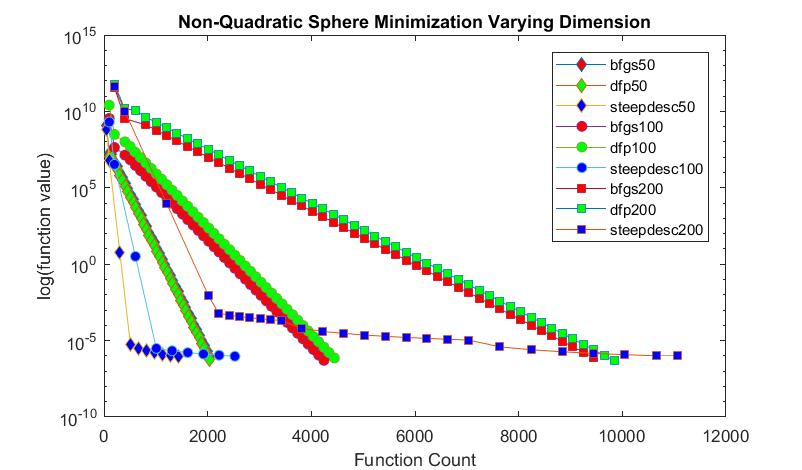
\includegraphics[width=9cm]{SphereDimenExploration1.jpg}
  \caption{Exploring how dimension affects the non-quadratic sphere}
  \label{fig:sdimen}
\end{figure}


\section{Algorithm}
\label{algorithm}
The algorithm used to get the results below utilizes two main functions. The first function's goal is to actually complete the minimization of the non-quadratic sphere. We first start with an initial starting point, $x_0$ (an $n$ dimensional column vector with random elements ranging from $0$ to $1$). Then we set our options for Matlab's fminunc function, where we set it to display a convergence graph. We also set the Hessian update option, the maximum number of functional evaluations allowed, the optimality tolerance, and the objective limit. We are only interested in achieving target values here, so we set the optimality tolerance to be arbitrarily small and the maximum number of function evaluations to be high, so that the algorithm does not stop trying to find the minimum value early. Next, we define a function that stores necessary variables, like function values for instance, for plotting purposes. Finally we define the objective function, which is the non-quadratic sphere as defined above. Overall, this function will take arguments: $n$ for the dimension, $\beta$ for the power, a target function value, and the Hessian update (a string), and returns the variables that we recorded. Note, some of the code to implement this was burrowed from \cite{MathWorks}.

The second algorithm is also a function but it uses the first algorithm to compute many runs with a specified value of $\beta$, but with different target values. The first step in this algorithm is to do many runs in of the first algorithm with a fixed $\beta$, but with a range of different target values. The runtime is gathered and stored for each run. Then we compute how many of these run-times were below a given run-time value, say run-time $t_0$, and divide this number by the total number of runs. This number is the number of successful problems (the number of problems that reached their target in time $t_0$ or less). This will then be repeated for a range of run-times, and all of these points will give data for a full cumulative run-time distribution plot for a specified value of $\beta$. This process will be repeated for each Hessian update variant, and the function will return the data for plotting. Finally, in another file, we run through many iterations of this algorithm and take the median of all of the iterations to present this as the final result in Figure \ref{fig:beta}, so that reproducing it is more likely.

\section{Results and Discussion}
\label{result}


\begin{figure*}[b]
\centering
  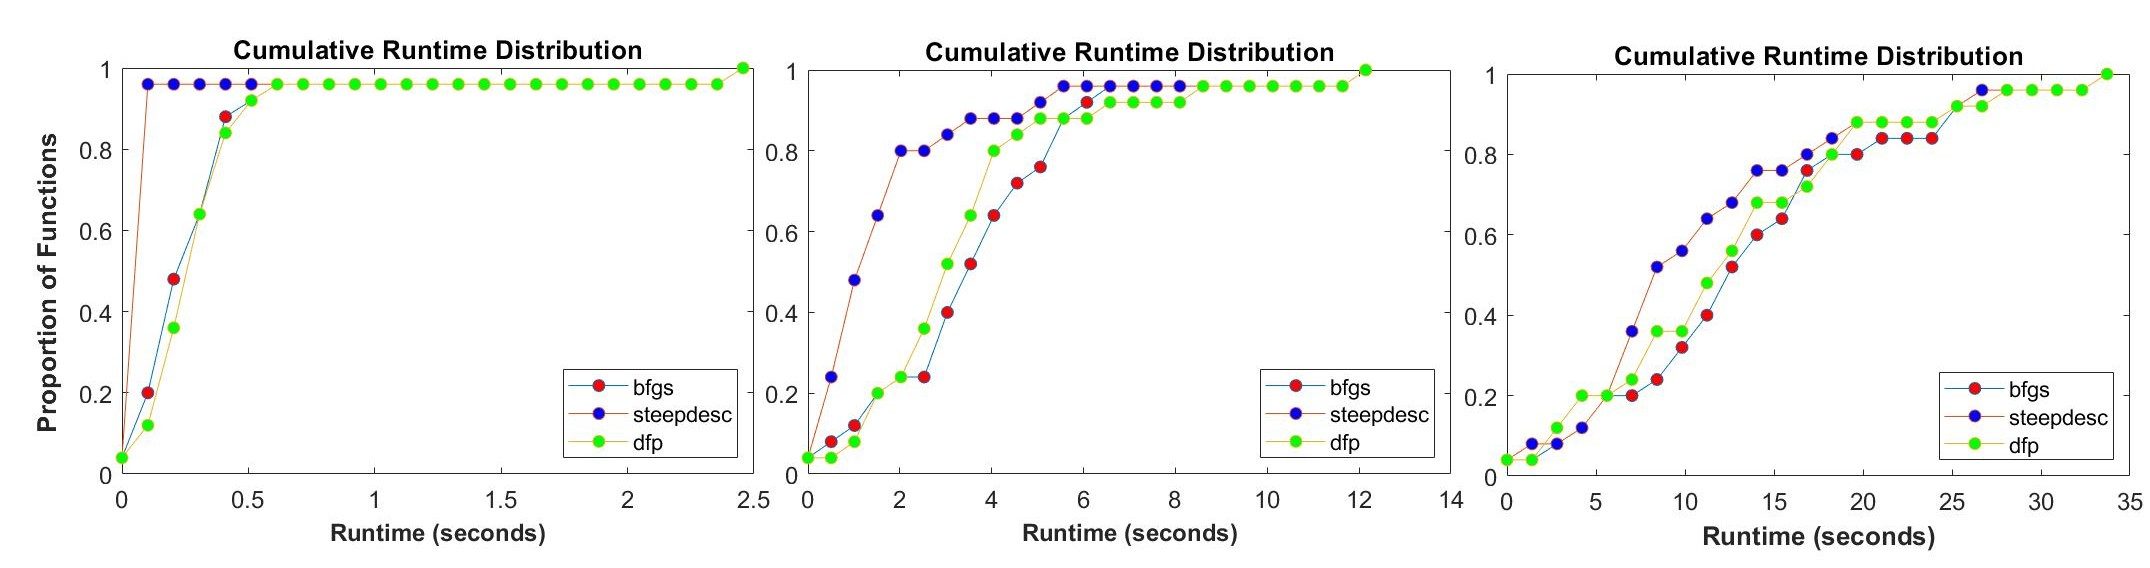
\includegraphics[height = 5cm, width=\linewidth]{CumDisBeta1.jpg}
  \caption{Cumulative run-time distribution plots. Left plot is for $\beta = 10$, middle plot is for $\beta = 25$, and the right plot is for $\beta = 40$. Dimension $n=50$ for all plots.}
  \label{fig:beta}
\end{figure*}

The first result is shown in Figure \ref{fig:sdimen}, and shows how increasing the dimension affects the non-quadratic sphere. In this case, we kept $\beta = 10$ constant, to accurately view the affect of the dimension on the problem. You can see that increasing the dimension of the problem did have the expected result, being that higher dimensions would simply increase function values and the number of function evaluations. When comparing the different Hessian updates, you can see that for both the cases of dimension $n = 50$ and $n = 100$, the steepdesc algorithm variant found the solution the fastest, while the other two were slightly more costly, by about the same amount. When the dimension is increased to $200$, you can see that the steepest decent algorithm gets closer to the optimal solution faster than the other two Hessian update variants, but then very slowly struggles to finally reach the optimal solution. This caused the other two Hessian updates to reach the target faster with less function evaluations. From this plot it seems like we can conclude that for lower dimensions the steepest descent Hessian update will be the least costly, where as for the higher dimensions, it seems like either the bfgs or dfp Hessian variant would be the least costly. Furthermore, for these higher dimensions, the bfgs updates seems to edge out the dfp Hessian variant a little bit in both the dimension $n=100$ and $n=200$ cases, so the bfgs update seems like the best option for higher dimensions.

Next, Figure \ref{fig:beta} shows three different cumulative run-time distribution graphs, each corresponding to their own value of $\beta$, with all three different Hessian update variants displayed for visual comparison. The first plot corresponds to $\beta = 10$, and shows that when using the steepdesc Hessian update variant, a large proportion of the functions reach their targets in time, and certainly more so than the other Hessian update variants, however it appears they all have the same result once the runtime passes a value of $0.5s$. This makes sense since, from Figure \ref{fig:sdimen}, it seems like the steepdesc Hessian variant usually works faster when function values are not too large. The middle plot shows a somewhat similar result, where steepdesc is better than the other two Hessian update variants, but it is not as much better this time, and after around $5s$, it seems like all Hessian update variants are roughly just as good as each other. The expectation here, as mentioned in \ref{sec:intro}, is that the bfgs and dfp Hessian variants would give better results for larger run-times, but when we look at the final plot on the right of Figure \ref{fig:beta}, we see that all Hessian update variants have roughly the same performance. The steepdesc variant still seems to do a bit better for smaller run-times, but the expectation that the bfgs and dfp variants would be better for larger run-times does not seem to hold. This may be because not enough target values, and thus data points, were considered, and so there is not enough information to properly display that the bfgs and dfp Hessian update variants could be slightly better than the steepdesc variant. It also may be that the dimension was not large enough (kept constant at $n=50$ here), so the steepdesc managed to perform well with all different values of $\beta$.



\section{Conclusion}
\label{con}
Finally, from the results observed in Figure \ref{fig:sdimen} and \ref{fig:beta}, the steepdesc Hessian update may be best for small dimensions and small powers (essentially for whenever function values are relatively smaller), as it minimizes the problem the fastest. That being said, it also appears that for higher dimensions it might get close to the minimum value, but struggle to actually reach it, so when trying to reach target values close to the minimum value, the bfgs or dfp Hessian updates may be better. Furthermore, for  larger values of $n$ and $\beta$, it was expected that the steepdesc Hessian update would have displayed this issue, and either the bfgs or dfp variants would likely have been better. Since this was not shown here, for future exploration, it may be of interest to increase the dimension and $\beta$, and observe if steepdesc is still as good as the other update variants. In regards to Figure \ref{fig:sdimen}, higher dimensions might be useful to make the conclusion that the steepdesc update variant is more costly for these higher dimensions stronger, as there is only one dimension value that shows this in Figure \ref{fig:sdimen}. 

\begin{thebibliography}{9}
\bibitem{MathWorks} 
MathWorks Output Functions,
\\\texttt{https://www.mathworks.com/help/releases/R2015b/optim/ug/output-functions.html}
\end{thebibliography}


\end{document}